\documentclass[14pt]{extbook}
\usepackage{multicol, enumerate, enumitem, hyperref, color, soul, setspace, parskip, fancyhdr} %General Packages
\usepackage{amssymb, amsthm, amsmath, bbm, latexsym, units, mathtools} %Math Packages
\everymath{\displaystyle} %All math in Display Style
% Packages with additional options
\usepackage[headsep=0.5cm,headheight=12pt, left=1 in,right= 1 in,top= 1 in,bottom= 1 in]{geometry}
\usepackage[usenames,dvipsnames]{xcolor}
\usepackage{dashrule}  % Package to use the command below to create lines between items
\newcommand{\litem}[1]{\item#1\hspace*{-1cm}\rule{\textwidth}{0.4pt}}
\pagestyle{fancy}
\lhead{Progress Quiz 10}
\chead{}
\rhead{Version B}
\lfoot{6232-9639}
\cfoot{}
\rfoot{Fall 2020}
\begin{document}

\begin{enumerate}
\litem{
First, find the equation of the line containing the two points below. Then, write the equation as $ y=mx+b $ and choose the intervals that contain $m$ and $b$.\[ (8, -11) \text{ and } (-2, 9) \]\begin{enumerate}[label=\Alph*.]
\item \( m \in [-4, -1] \hspace*{3mm} b \in [-5.46, -4.84] \)
\item \( m \in [2, 5] \hspace*{3mm} b \in [11.32, 13.22] \)
\item \( m \in [-4, -1] \hspace*{3mm} b \in [-19.03, -18.73] \)
\item \( m \in [-4, -1] \hspace*{3mm} b \in [3.74, 6.39] \)
\item \( m \in [-4, -1] \hspace*{3mm} b \in [10.86, 12.91] \)

\end{enumerate} }
\litem{
Find the equation of the line described below. Write the linear equation as $ y=mx+b $ and choose the intervals that contain $m$ and $b$.\[ \text{Parallel to } 8 x - 9 y = 7 \text{ and passing through the point } (-8, -7). \]\begin{enumerate}[label=\Alph*.]
\item \( m \in [0.7, 0.94] \hspace*{3mm} b \in [-0.03, 0.36] \)
\item \( m \in [1.1, 2] \hspace*{3mm} b \in [-0.03, 0.36] \)
\item \( m \in [-0.91, -0.61] \hspace*{3mm} b \in [-14.12, -14.03] \)
\item \( m \in [0.7, 0.94] \hspace*{3mm} b \in [-0.26, 0.01] \)
\item \( m \in [0.7, 0.94] \hspace*{3mm} b \in [0.55, 1.14] \)

\end{enumerate} }
\litem{
Find the equation of the line described below. Write the linear equation as $ y=mx+b $ and choose the intervals that contain $m$ and $b$.\[ \text{Parallel to } 8 x + 7 y = 3 \text{ and passing through the point } (-8, -9). \]\begin{enumerate}[label=\Alph*.]
\item \( m \in [-1.31, -1.04] \hspace*{3mm} b \in [15.14, 23.14] \)
\item \( m \in [-1.31, -1.04] \hspace*{3mm} b \in [-20.14, -13.14] \)
\item \( m \in [1, 1.15] \hspace*{3mm} b \in [-0.86, 2.14] \)
\item \( m \in [-1.31, -1.04] \hspace*{3mm} b \in [-3, 0] \)
\item \( m \in [-0.94, -0.58] \hspace*{3mm} b \in [-20.14, -13.14] \)

\end{enumerate} }
\litem{
First, find the equation of the line containing the two points below. Then, write the equation as $ y=mx+b $ and choose the intervals that contain $m$ and $b$.\[ (2, -5) \text{ and } (7, 10) \]\begin{enumerate}[label=\Alph*.]
\item \( m \in [1, 7] \hspace*{3mm} b \in [-16, -9] \)
\item \( m \in [1, 7] \hspace*{3mm} b \in [8, 15] \)
\item \( m \in [-11, 1] \hspace*{3mm} b \in [25, 38] \)
\item \( m \in [1, 7] \hspace*{3mm} b \in [-9, 0] \)
\item \( m \in [1, 7] \hspace*{3mm} b \in [-3, 4] \)

\end{enumerate} }
\litem{
Write the equation of the line in the graph below in Standard form $Ax+By=C$. Then, choose the intervals that contain $A, B, \text{ and } C$.
\begin{center}
    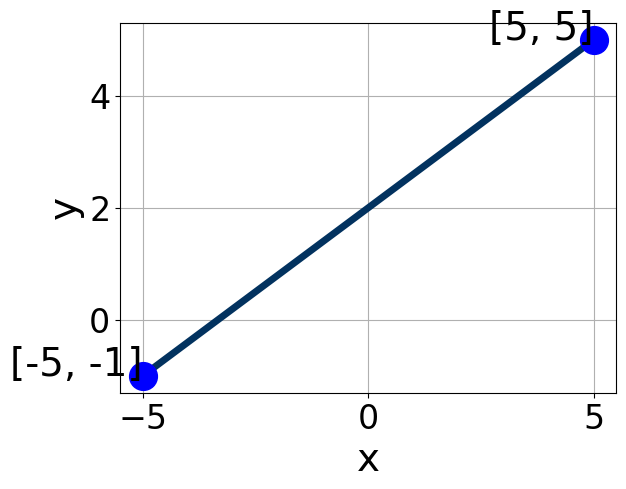
\includegraphics[width=0.5\textwidth]{../Figures/linearGraphToStandardCopyB.png}
\end{center}
\begin{enumerate}[label=\Alph*.]
\item \( A \in [2.3, 3.6], \hspace{3mm} B \in [4.54, 6.34], \text{ and } \hspace{3mm} C \in [8.6, 10.8] \)
\item \( A \in [2.3, 3.6], \hspace{3mm} B \in [-6.2, -4.41], \text{ and } \hspace{3mm} C \in [-12.2, -9.5] \)
\item \( A \in [-1.8, 0.1], \hspace{3mm} B \in [-0.26, 1.69], \text{ and } \hspace{3mm} C \in [1.6, 3.9] \)
\item \( A \in [-1.8, 0.1], \hspace{3mm} B \in [-2.41, 0.59], \text{ and } \hspace{3mm} C \in [-3.7, -1.9] \)
\item \( A \in [-5.5, -0.8], \hspace{3mm} B \in [4.54, 6.34], \text{ and } \hspace{3mm} C \in [8.6, 10.8] \)

\end{enumerate} }
\litem{
Solve the equation below. Then, choose the interval that contains the solution.\[ -14(-18x -17) = -8(6x + 2) \]\begin{enumerate}[label=\Alph*.]
\item \( x \in [-1.16, -0.98] \)
\item \( x \in [0.71, 0.82] \)
\item \( x \in [-0.95, -0.78] \)
\item \( x \in [-0.84, -0.69] \)
\item \( \text{There are no real solutions.} \)

\end{enumerate} }
\litem{
Solve the linear equation below. Then, choose the interval that contains the solution.\[ \frac{-3x -3}{7} - \frac{4x -7}{6} = \frac{-4x + 5}{4} \]\begin{enumerate}[label=\Alph*.]
\item \( x \in [-10.5, -8.5] \)
\item \( x \in [-2.17, 1.83] \)
\item \( x \in [-6.38, -4.38] \)
\item \( x \in [-30.88, -26.88] \)
\item \( \text{There are no real solutions.} \)

\end{enumerate} }
\litem{
Solve the linear equation below. Then, choose the interval that contains the solution.\[ \frac{9x + 6}{5} - \frac{-5x + 6}{6} = \frac{9x + 3}{4} \]\begin{enumerate}[label=\Alph*.]
\item \( x \in [-1.5, 0.3] \)
\item \( x \in [-4.1, -2.3] \)
\item \( x \in [6.5, 8.7] \)
\item \( x \in [0.5, 2] \)
\item \( \text{There are no real solutions.} \)

\end{enumerate} }
\litem{
Write the equation of the line in the graph below in Standard form $Ax+By=C$. Then, choose the intervals that contain $A, B, \text{ and } C$.
\begin{center}
    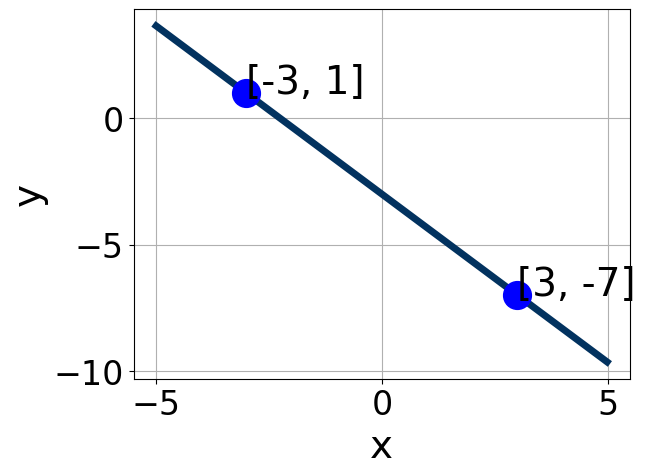
\includegraphics[width=0.5\textwidth]{../Figures/linearGraphToStandardB.png}
\end{center}
\begin{enumerate}[label=\Alph*.]
\item \( A \in [3.7, 4.7], \hspace{3mm} B \in [-4.92, -2.14], \text{ and } \hspace{3mm} C \in [9, 11] \)
\item \( A \in [0.5, 3.7], \hspace{3mm} B \in [0.7, 2.07], \text{ and } \hspace{3mm} C \in [-3, 0] \)
\item \( A \in [3.7, 4.7], \hspace{3mm} B \in [2.89, 4.99], \text{ and } \hspace{3mm} C \in [-11, -6] \)
\item \( A \in [-4.4, -2.6], \hspace{3mm} B \in [-4.92, -2.14], \text{ and } \hspace{3mm} C \in [9, 11] \)
\item \( A \in [0.5, 3.7], \hspace{3mm} B \in [-1.5, 0.65], \text{ and } \hspace{3mm} C \in [2, 5] \)

\end{enumerate} }
\litem{
Solve the equation below. Then, choose the interval that contains the solution.\[ -19(-10x + 6) = -8(13x -2) \]\begin{enumerate}[label=\Alph*.]
\item \( x \in [0.18, 0.41] \)
\item \( x \in [0.34, 0.83] \)
\item \( x \in [1.11, 1.55] \)
\item \( x \in [-0.82, 0.17] \)
\item \( \text{There are no real solutions.} \)

\end{enumerate} }
\end{enumerate}

\end{document}